\documentclass[10pt,a4paper]{article}
\usepackage[utf8]{inputenc}
\usepackage{amsmath}
\usepackage{amsfonts}
\usepackage{amssymb}
\usepackage{graphicx}
\usepackage{array}
\usepackage{tabu}
\usepackage{listings}
\usepackage{color}
\usepackage{hyperref}
\usepackage{multirow}
\usepackage[table]{xcolor}

\DeclareMathOperator*{\argmin}{arg\,min}
\DeclareMathOperator*{\argmax}{arg\,max}

\lstset{language=Java,
  showspaces=false,
  showtabs=false,
  breaklines=true,
  showstringspaces=false,
  breakatwhitespace=true,
  commentstyle=\color{green},
  keywordstyle=\color{magenta},
  stringstyle=\color{red},
  identifierstyle=\color{blue},
  basicstyle=\ttfamily,
}

\begin{document}

% title page initialization has to  be inside documents,  so that we can use tabular in author
\title{Predicting School Performance \\ in \\ Portuguese Youth}
\author{
\begin{tabular}{lcc}
\hline
Name & Matriculation Nr. & Contribution\\ \hline
    Skála Matouš & N1602866H & 17 \%\\
Arcenas Carlos Alberto Lagdameo  & N1604152E & 17 \%\\
Widmer Christian  & N1602590C & 17 \%\\
Hunshamar Bjørnar & N1602951E & 17 \%\\
Groschupp Friederike Juliane & N1602589L & 17 \%\\
Efrem Afework Yared & N1603716J & 17 \% \\ \hline
\end{tabular}
}
\date{\today}


\maketitle
\newpage

\tableofcontents
\newpage

\begin{abstract}
    The goal of this project was to explore the usage and techniques of different data mining techniques, and compare their advantages and disadvantages by using a data set sourced from real-world studies. The data set itself was created through the school results of 649 students from a Portuguese secondary school, and a questionnaire that was provided to these students. The grades and absences of the students were extracted from each student's school reports, while the questionnaire was used to gather demographic, social, and school related features. In this report, the students were classified based on their average grade across the three terms reported. In particular, binary classification was used to determine whether the student's grade was ``Above'' or ``Below'' average, and 5-level-classification was used to assign one of five labels from ``Very Good'' to ``Fail'' to the average grade. In order to classify the students, four different data mining techniques were applied: k-Nearest Neighbour, Decision Trees, Naïve Bayes, and Neural Networks. In addition to classifying the average grade, this project also aimed to predict the average grade of a student through the use of linear regression by way of feature selection and calculation and through neural networks. These methods were trained and tested by using separate training and test sets calved from the full data set. The records for the test set were chosen randomly and consist of one-third of all students from the full data set. The algorithms chosen were either from scratch or used various machine-learning libraries such as scikit-learn \cite{sklearn} and Google's TensorFlow \cite{tf}.The results of these custom-made implementations were compared to the results from the popular Java library Weka \cite{weka}. Finally, the calculations from all methods were analyzed, and it was determined if accurate classifications and regressions can be made from this data set. 
\end{abstract} 

\newpage

\section{Problem Description}
\subsection{Motivation}
The performance of students in an academic setting is almost always measured through the use of a raw or weighted score summarizing the success and compliance of a student's work to set benchmarks across a certain period. While common perception regarding a student's performance typically revolves around the number of hours spent studying for assessments, it is understood that many other factors can feed into determining whether a student performs at an academically high or low level. These factors range from simply-described features such as a student's biological sex to more varied and complex phenomena such as a student's family's education status. Given this wide catchment, forming an efficient and targeted approach to improving the scores of those who may be under-performing will have to take all of these factors into account. With the advent of data mining, it would be possible to determine and direct sources of external help, from simple efforts such as the placement of students in supplementary classes, to bigger efforts such as the mobilization of governmental and national resources to help support what would otherwise be under-performing students.


\subsection{Problem Definition}
The database of student records, describing Portuguese student information and performance, was sourced from two public schools in Portugal, covering the 2005-2006 academic year. The database was split into two different data sets, corresponding to the specific subject these grades were sourced from. The subjects covered were mathematics, and studies of the Portuguese language. There are 1,046 instances across both data sets, with Portuguese results contributing 650 records, and Mathematics picking up the rest, each describing a specific student, with 382 students having records across both data sets. Each record is described by a manner of 30 attributes covering various demographic qualities of a student, from basic biological information like a student's sex and age, to more environmental factors such as a student's access to Internet and the quality of a student's familial relationships. In addition to the demographic qualities, each record contains three scores corresponding to the student's performance in a certain subject at the end of the first, second and third period of grading. Table \ref{table:attributes} includes the names, ranges and abbreviations of each attribute in the data set. The original data set can be obtained from \href{https://archive.ics.uci.edu/ml/datasets/student+alcohol+consumption}{here} . With this data set, this experiment aims to predict the band of arbitrary student's upcoming average grade with their demographic information and previous grades through the use of binary and five-class classifiers. In addition, in a similar vein, this report aims to see if a numerical value for the average grade can be obtained with the same information through linear regression.

\begin{table}
\center
\rowcolors{2}{gray!35}{}
\begin{tabular} {m{1em} m{1.5cm} m{9cm}} 
 \hline
 No. & Attribute & Range of values \\
 \hline
 1 & school & ``Gabriel Pereira''=GP, ``Mousinho da Silveira''=MS \\ 
 2 & sex & female=F, male=M \\ 
 3 & age & number from 15 to 22 \\
 4 & address & urban=U, rural=R \\
 5 & famsize & ``less than or equal to 3''=LE3, ``greater than 3''=``GT3'' \\
 6 & Pstatus & ``parents living together''=T, ``parents living apart''=A \\
 7 & Medu & ``no education''=0, ``up to 4th grade''=1, ``between 5th and 9th grade''=2, ``secondary education''=3, ``higher education''=4 \\
 8 & Fedu & ``no education''=0, ``up to 4th grade''=1, ``between 5th and 9th grade''=2, ``secondary education''=3, ``higher education''=4 \\
 9 & Mjob & teacher=teacher, ``care related''=health, ``civil (e.g. administrative or police)''=services, ``at home''=at\_home, other=other \\
 10 & Fjob & teacher=teacher, ``care related''=health, ``civil (e.g. administrative or police)''=services, ``at home''=at\_home, other=other \\
 11 & reason & ``close to home''=home, ``school reputation''=reputation, ``course preference''=course, other=``other'' \\
 12 & guardian & mother=mother, father=father, other=other \\
 13 & traveltime & \textless15min=1, 15-30min=2, 30min-1hour=3, \textgreater1hour=4 \\
 14 & studytime & \textless2hours=1, 2-5hours=2, 5-10hours=3, \textgreater10hours=4 \\
 15 & failures & 0\textless n\textless3=n, n\textgreater3=4 \\
16 & schoolsup & yes=yes, no=no \\
17 & famsup & yes=yes, no=no \\
18 & paid & yes=yes, no=no \\
19 & activities & yes=yes, no=no \\
20 & nursery & yes=yes, no=no \\
21 & higher & yes=yes, no=no \\
22 & internet & yes=yes, no=no \\
23 & romantic & yes=yes, no=no \\
24 & famrel & rating from ``very bad''=1 to ``excellent''=5 \\
25 & freetime & rating from ``very low''=1 to ``very high''=5 \\
26 & goout & rating from ``very low''=1 to ``very high''=5 \\
27 & Dalc & rating from ``very low''=1 to ``very high''=5 \\
28 & Walc & rating from ``very low''=1 to ``very high''=5 \\
29 & health & rating from ``very bad''=1 to ``very good''=5 \\
30 & absences & number from 0 to 93 \\
 \hline
\end{tabular}
\caption{Names, ranges and abbreviations of each attribute in the data set.}
\label{table:attributes}
\end{table}
\subsubsection{Data set compilation}
As mentioned in the previous section, the data set was built from two sources. The first source was the official school reports that included the three period grades and each student's number of absences. The second source was the results of a questionnaire with 37 questions designed to extract several demographic (e.g. father's education), social/emotional (e.g. alcohol consumption), and school related variables (e.g. study time). The specific range and definition of each of these attributes are shown in Table 1.

\subsection{Related Works and Subsequent Approaches}
The data set was initially created by Paulo Cortez and Alice Silva from the University of Minho in Portugal for their report: Using Data Mining To Predict Secondary School Student Performance \cite{cortez2008}. Since then, the data set has also been used as a source for other papers, including the report Predicting Student Alcohol Consumption by Fabio Pagnotta and Mohammad Amran Hossain \cite{alcohol}. 
Unlike the original study, this experiment did not aim to predict the final ``G3'' grade based on previous grades and social attributes, but instead to predict the average grade using just the social attributes. For this reason the grades as reported from all three periods were merged into one average grade. 
This allowed for the grouping of the students in regards to their average grade in the following ways:
\begin{enumerate}
    \item via Binary Classification: Students can be classified with one of two class labels regarding whether their grade is below or above average. ``Above'' if $ grade  >  12$  and ``Below'' if  $ grade \le  12$, as shown in table \ref{table:binaryClassification}.
    \item via 5-Level Classification: Students can be assigned to one of 5 groups according to their average grade in ``Very Good'', ``Good'', ``Satisfactory'', ``Sufficient'', and ``Fail'', as shown in table \ref{table:5levelClassification}.
\end{enumerate}

\begin{table}[h]
\center
\begin{tabular}{cccc}
\hline
    Class & Condition & Count & Percentage \\
    \hline
    Above & $ grade  >   12 $ & 303 & 48\% \\
    Below & $ grade  \le  12 $ & 329 & 52\% \\
    \hline
\end{tabular}
\caption{Selecting 2 class labels regarding student's average grade}
\label{table:binaryClassification}
\end{table}
\begin{table}[h]
\center
\begin{tabular}{cccc}
\hline
    Class & Condition & Count & Percentage \\
    \hline
    Very Good & $ 16 \le grade \le 20 $ & 47 & 7.4 \% \\
    Good & $ 14\le grade < 16 $  & 89 & 14.1 \% \\
    Satisfactory & $ 12\le grade < 14 $ & 167 & 26.4 \% \\
    Sufficient & $ 10\le grade < 12 $ & 187 & 29.6 \% \\
    Fail & $ 0 \le grade < 10 $  & 142 & 22.5 \%\\
    \hline
\end{tabular}
\caption{Selecting 5 class labels regarding student's average grades}
\label{table:5levelClassification}
\end{table}
%Add table and histograms
\section{Approach}	
	\subsection{Data Preprocessing}
	Data preprocessing is an essential part of data mining, as it ensures that the data analysis can be run smoothly and that the acquired results are reliable and not blurred by outliers or missing values. As the data set was already used for data mining in other studies, it was found to be in good condition. Nevertheless, some adjustments were necessary.
	\\
	\\ These adjustments included:
	\begin{itemize}
	    \item Data cleaning: While going through the data sets, it was realized that some students had relatively high grades in Term 1 and occasionally in Term 2, but had a grade of 0 in the third term. Given that, it was assumed that, in the most likely case, the students dropped out of the school programme. To make sure that these data points do not negatively affect the results, their records were deleted from the database.
	    \item Data transformation: Most of the algorithms implemented in this experiment only work with numbers, not with nominal attributes. There are four attributes in the database that are nominal: ``Mother's job'', ``father's job'', ``reason to choose this school'' and the ``guardian''. It was decided that transformation of the parent's job attributes to binary attributes—to ``at home'' and ``at work'' was necessary. The values the attributes could take before were not distinct enough, and that not much information would be lost with the transformation. The other two attributes were transformed through binarization: that is, the splitting up in binary attributes for every of their possible values. Additionally, most of the binary attributes did not have 0 and 1 as their only values, rendering a transformation necessary for these attributes as well..
	   % \item Introduction of new attributes: As we decided to predict the average grade and the change of the grade from term 1 to term 2 of a student, we calculated the values from the grades of term 1 to term 2 and introduced them as new attributes.
	    \end{itemize}
	    
	    \subsubsection{Feature sub-selection}
	    Initially the CfsSubsetEval filter provided by Weka was used to select the features to be used in each of the algorithms. The filter ranks the possible subsets by considering the individual impact of each feature and the redundancy between them. However, it was discovered that a sub-selection of attributes had little to no effect on the accuracy of the classifiers. This is likely because many techniques apply the embedded approach, i.e. feature sub-selection from all features present in the data set occurs naturally as part of the data analysis algorithm.
	    
	    \subsubsection{Distribution of training and test Set}
	    After the data cleaning, the full data set with 632 instances was shuffled and split into a training set with 422 records, i.e. two thirds (67 \%) of the original data set; and a test set containing 210 data objects, i.e. one third (33 \%) of the full data set. The split is shown in Table 4.
	    
	    \begin{table}[h]
	        \centering
	        \begin{tabular}{cccc}
	        \hline
	            Class &  Training set & Test set & Sum\\ \hline
	            Above & 210 & 93  & 303 \\
	            Below & 212 & 117 & 329\\ \hline
	            Sum & 422 & 210 & 632 \\
	            \hline
	        \end{tabular}
	        \caption{Distribution of binary classes among training and test set}
	        \label{tab:binClassDistribution}
	    \end{table}
	    
	    Table \ref{tab:binClassDistribution} shows the distribution of records according to their binary class label in the training and test set. In our case 49\% of the training set and 44\% of the test set have the class label ``Above''. Table \ref{tab:multiClassDistribution} shows the distribution when using 5 class labels ranging from ``Very Good'' to ``Fail''.
	    
	    \begin{table}[h]
	        \centering
	        \begin{tabular}{cccc}
	        \hline
	            Class &  Training set & Test set & Sum\\ \hline
	            Very Good & 31  & 16 & 47 \\
	            Good & 67 & 22 & 89 \\
	            Satisfactory & 112  & 55 & 167 \\
	            Sufficient & 116 & 71 & 187 \\
	            Fail & 96  & 46 & 142 \\ \hline
	            Sum & 422 & 210 & 632 \\
	            \hline
	        \end{tabular}
	        \caption{Distribution of 5 label classes among training and test set}
	        \label{tab:multiClassDistribution}
	    \end{table}

	\subsection{Algorithms}
	Across this experiment, five different data mining techniques were chosen to analyze the aims of the experiment. The techniques used are Linear Regression, Naive Bayes Classifiers, k-nearest Neighbours, Artificial Neural Networks, and Decision Trees. In the following sections, each of the implemented algorithms is described in detail.
	
	\subsubsection{Linear Regression (LR)}
	Regression is a predictive technique where the target variable is continuous. The linear regression algorithm (LR) attempts to predict a dependent variable \(y\) as a linear combination of inputs \(x_1, x_2, ..., x_n\):
	\begin{align}
	y = w_0 + w_1x_1 + w_2x_2 + ... + w_nx_n
	\end{align}
	where \(w_0, w_1, ..., w_n\) are known as regression coefficients or weights.

	
	The Ordinary Least Squares (OLS) estimator is the most common method for solving the linear regression problem.
	\\
	Given data set \({(x_p, d_p)}^P_{p=1}\). Let \(y_p\) be the predicted output for \(\textbf{x}_p = (x_{p,1}, x_{p,2}, ..., x_{p,n})\). Equation (1) can be written in matrix form: \(\textbf{Xw} = \textbf{y}\).
	OLS method minimizes the sum of squared residuals and leads to the following expression for the estimated value of the unknown parameter \(\textbf{w}\):
	\begin{align}
	\textbf{ŵ} = (\textbf{X}^T\textbf{X})^{-1}\textbf{X}^T\textbf{d}
	\end{align}

	\subsubsection{Naïve Bayes Classifier (NB)}
	The Naïve Bayes classifier (NB) is a simple but popular classification method. It predicts the probability of an unknown instance to belong to class $C$ based on the attributes $A$; in other words, the goal is to find the value $x$ of class $C$ that maximizes the posterior probability of $C$ given $A$ $P(C|A)$ (3). In order to do so, the method makes the assumption that each attribute is independent of the others (4). This assumption is called the Naïve Bayes assumption.
	\begin{align}
			x_{max} = \argmax_{x \in C} &= P(x|A_1, ..., A_n) \\
			&= \frac{P(A_1, ..., A_n|x)P(x)}{P(A_1, ..., A_n)} \\
			&= P(A_1, ..., A_n|x)P(x) \\
			&= P(A_1|x) \cdot ... \cdot P(A_n|x) \cdot P(x) \\
			&= \prod_{i = 1}^{n}P(A_i|x) \cdot P(x)
	\end{align}
	
	\subsubsection{k-Nearest Neighbor (kNN)}
	The k-Nearest Neighbor algorithm (kNN) is an instance-based classifier that is based on comparing similarities between instances. kNN can be used for regression and classification. The similarity is measured by using a distance metric, such as the Euclidean distance between instances. Instances with smaller distances are considered to be more similar. The parameter $k$ specifies the number of neighbors used for the regression or classification. Typically, $k$ takes small integer values. When a new instance is introduced, the algorithm computes the distance to all existing instances and selects the nearest neighbors, with quantity specified by $k$.   
	\begin{itemize}
		\item When used as a classification algorithm, the class of the unknown instance will be determined by majority vote of the nearest neighbors, i.e. the new instance will be assigned to the class most common among its neighbors. 
		\item When used as a regression algorithm, the value of the unknown instance is found as the average of the value of its neighbors.	 
	\end{itemize}
	
	For the best accuracy it is important to determine the optimal value for the parameter $k$. While a small value for $k$ makes the result prone to noise and outliers, a larger value means the k-nearest neighbors include instances that have little similarity with the unknown one. A possible solution is to not give every neighbor one vote, but to weigh every neighbor based on the distance to the new instance. For instance, a weight of $\frac{1}{d}$ means that closer instances have more weight than further ones. 
	\\	
	Additionally, the chosen distance metric can also have a high impact on the accuracy. One possible distance metric is the Euclidean distance, however this requires all attributes to be normalized. With that considered, this report chose to use the Euclidean distance, prompting the need to normalize each attribute.

	\subsubsection{Artificial Neural Networks (NN)}
	An artificial neural network (NN) is a machine-learning approach that is based on the biological neural network of the human brain. This experiment implemented a multilayer perceptron network (MLP) which is a feed-forward neural network. The feed-forward NN consists of multiple layers, with each layer made up of multiple artificial neurons, also known as perceptrons. Each perceptron of one layer is linked to each perceptron of the next layer. These links are weighted, and during the learning phase the network is learning by adjusting the weights on each link to predict the class of the input samples. A supervised learning algorithm known as backpropagation is used, along with the gradient descent optimization algorithm.
	The MLP in this experiment has 35 input nodes, with each corresponding to one of the 35 attributes found in the data set.
	
	This experiment implemented two types of ANN: one for regression, to predict the grade of a student as a real number; and one for classification, to predict the grade of a student as within one of the five bands as described earlier.
	
	\subsubsection{Decision Trees (DT)}
	The idea of decision trees (DT) is to introduce decision nodes that categorize the instances based on the value of one attribute per node, thereby dividing the data set into multiple subsets. Each of the new subsets becomes more homogeneous, meaning. it contains less different classes. The goal is to achieve a homogeneous class distribution—however, this is prone to over-fitting. 
	To be able to compare different nodes and find possible decision nodes a metric was needed to measure the node impurity, i.e. how many different classes are in one node. In fact there are several ways to measure node impurity, for example the Gini Index or Entropy.
	
	The experiment's implementation of decision trees in Python used the sklearn library that implements an optimized version of the CART algorithm and chooses the best split according to the Gini Index:
	
	When a node $p$ is split into $k$ partitions, the quality of the split $GINI_{split}$ is computed as,
	\begin{equation}
	    GINI_{split}(p) = \sum_{i = 1}^{k} \frac{n_i}{n} GINI(i)
	\end{equation}
	 where $n_i$ is the number of records at partition $i$ and $n$ the number of records at node $p$. 
	 
	 For each of the partitions $i$ the Gini Index is computed as,
	 \begin{equation}
	     GINI(i) = 1 - \sum_{j}^{n_c}(P(j|i))^2
	 \end{equation}
	 where $P(j|i)$ is the relative frequency of class $j$ at partition $i$ and $n_c$ the number of classes. 
	
	% Explanation regarding minimum/maximum values
	
	

	
\section{Implementations}
\subsection{Linear Regression}
The experiment's linear regression algorithm was implemented in Python with the use of the scikit-learn package. On the Weka end, the LinearRegression classifier was used.

\subsection{Naîve Bayes}
Similar to the linear regression implementation, the experiment's naîve Bayes classifier was implemented in Python with the use of the scikit-learn package. On the Weka end, the NaiveBayes classifier was used.

\subsection{k-Nearest Neighbour}
The kNN algorithm was implemented from scratch in Java without using any external libraries and achieved comparable results to the kNN classifier as provided by Weka. The result comparison between the experiment's implementation and Weka can be found in the next section.
\\
\\Because the kNN algorithm implemented is a ``lazy learner'' there is no typical ``learning phase'' like other techniques (e.g. ANNs) have. Instead, the ``learning'' is performed each time when an unknown instance is passed to the algorithm. However, there are still two phases of the kNN algorithm that can be differentiated.
In the first phase all training instances are loaded and each record stored as an Instance object. Listing \ref{lst:kNNInstance} shows the implementation of the instance object in Java. In the second phase each test instance is taken from the test set and the euclidean distance is calculated, as shown in Listing \ref{lst:kNNEuclidean}. Subsequently, the k nearest neighbours are chosen and the class label of the test instance is determined by the most common class label among the neighbours.

\begin{lstlisting}[language=Java, caption={POJO to store instances}, label=lst:kNNInstance]
public class Instance implements Comparable<Instance> {
	public double[] attributes;
	public String classValue;
	//Will be set when calculating nearest neighbour
	public double distance;
	
	public Instance(double[] attributes, String classValue) {
		super();
		this.attributes = attributes;
		this.classValue = classValue;
	}	
}
\end{lstlisting}

\begin{lstlisting}[language=Java, caption={Calculate euclidean distance}, label=lst:kNNEuclidean]
private double calculateEuclidieanDistance(Instance from, Instance to) {
		double distance = 0.0;
		for(int i = 0; i < from.attributes.length; i++) {
			distance += Math.pow(from.attributes[i] - to.attributes[i], 2);
		}
		return Math.sqrt(distance);
	}
\end{lstlisting}

\subsection{Artificial Neural Networks}
The regression was implemented in Python, using Google's TensorFlow library for ANN, while the classifier was implemented using Matlab's Neural Pattern Recognition tool. The 

\subsection{Decision Trees}
The Decision Tree classifiers were implemented in Python using the DecisionTreeClassifier() class provided by the sklearn library. This was used both for the 5-level classifier and the binary classifier. After experimenting with different values in the object constructor, it was discovered that the default values gave the best results. The Gini impurity was used to measure the quality of the split, and had no limit on the number of features, maximum depth and and amount of leaf nodes. On the Weka end, the J48 classifier was used for comparison.
\section{Results}
\subsection{Linear Regression}
The results obtained from the linear regression implementation are equivalent with those obtained from Weka.

\begin{table}[h!]
  \centering
  \begin{tabular}{lll}
  \hline
  \textbf{Metric} & \textbf{scikit-learn} & \textbf{Weka} \\
  \hline
  Mean Square Error & 5.07 & 5.07 \\
  Mean Absolute Error & 1.77 & 1.77\\
  Relative Absolute Error & 86.67 \% & 86.67 \%\\
  \hline
  \end{tabular}
  \caption{Linear regression results}
  \label{tab:table3}
\end{table}

\begin{figure}[h!]
    \centering
    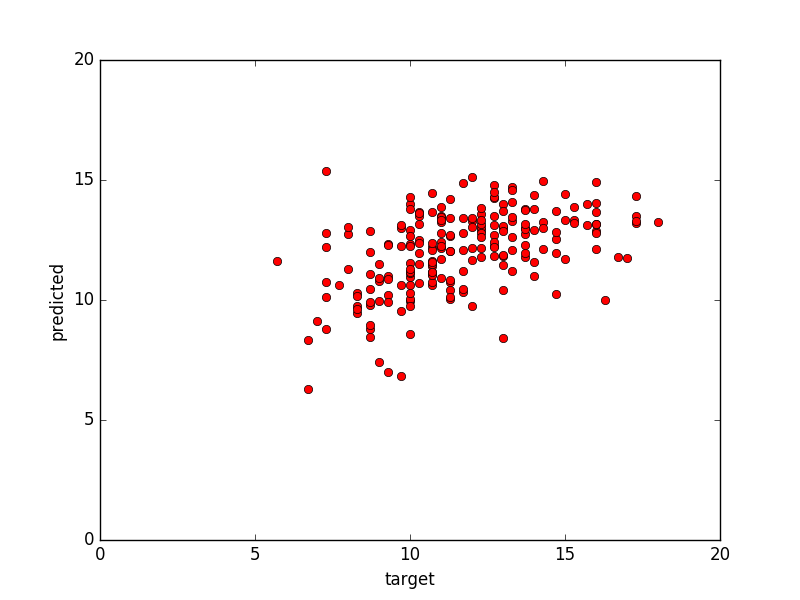
\includegraphics[width = 0.9\linewidth]{l_regression_test.png}
    \caption{Regression visualization showing predicted vs target values}
    \label{fig:fig1}
\end{figure}

\subsection{Naïve Bayes}
The implemented algorithm turned out to be unsuitable for this task as the results were not satisfactory. However, the results given by Weka were much better, probably due to slightly different implementation.

\subsubsection{Binary Classification}
For binary classification, the accuracy of our code is 63.81 \%. The accuracy of Weka's classifier is 66.19 \%.
\begin{table}[h]
\begin{center}
  \begin{tabular}{c|cc}
  & \multicolumn{2}{c}{\textbf{Target Class}} \\
 \textbf{Output} & Below & Above\\ \hline
  Below & 58 & 17 \\
  Above & 59 & 76
\end{tabular}
\quad
\begin{tabular}{c|cc}
  & \multicolumn{2}{c}{\textbf{Target Class}} \\
 \textbf{Output} & Below & Above\\ \hline
  Below & 64 & 18 \\
  Above & 53 & 75
\end{tabular}
\caption{Left table: Our Results for $k = 1$; Right table: Weka's results for $k = 2$ }
\label{tab:kNNbin}
\end{center}
\end{table}

\subsubsection{Multilevel Classification}
In multilevel classification, the accuracy of our code is only 19.52 \%, while Weka's classifier achieved the accuracy of 31.90 \%.
\begin{table}[h]
  \begin{tabular}{l|ccccc}
     & \multicolumn{5}{c}{\textbf{Target Class}} \\ 
  \textbf{Output} & Very Good & Good & Satisfactory & Sufficient & Fail \\  \hline
  Very Good  & 15 & 19 & 49 & 56 & 21\\
     Good & 0 & 2 & 2 & 0 & 0\\
     Satisfactory & 1 & 0 & 0 & 3 & 0\\
     Sufficient & 0 & 0 & 3 & 7 & 8\\
     Fail & 0 & 1 & 1 & 5 & 17\\
  \end{tabular}
  \caption{Confusion matrix of our own implementation}
  \label{tab:kNNmultiOwn}
\end{table}

\begin{table}[h]
  \begin{tabular}{l|ccccc}
     & \multicolumn{5}{c}{\textbf{Target Class}} \\ 
  \textbf{Output} & Very Good & Good & Satisfactory & Sufficient & Fail \\  \hline
  Very Good  & 2 & 2 & 6 & 5 & 0\\
     Good & 5 & 8 & 19 & 6 & 3\\
     Satisfactory & 6 & 8 & 18 & 32 & 3\\
     Sufficient & 2 & 3 & 10 & 16 & 17\\
     Fail & 1 & 1 & 2 & 12 & 23\\
  \end{tabular}
  \caption{Confusion matrix outputted by Weka's algorithm}
  \label{tab:kNNmultiWeka}
\end{table}

\subsection{k-Nearest Neighbor}
As mentioned in section 3.1. the kNN algorithm was implemented in Java and achieved similar results as the kNN algorithm provided by Weka. In this section the confusion matrices for both techniques for both classification techniques, i.e. binary and multilevel classification, are shown and compared. 
\subsubsection{Binary Classification}
For binary classification our implementation achieves the highest and equal accuracy for $ k = 1 $ and $ k = 2$. Interestingly, for both $k$ values we get the same number of 129 correctly and 81 incorrectly classified results of 210 test instances i.e. an accuracy of 61.43\%. However, the F1 scores differentiate slightly for both $k$ values with 61.3 \% for $k = 1$ and 60.7 \% for $k = 2$. \\
\\
Weka's nearest neighbor classifier performs best with $k = 2$. It classifies 137 correctly and 73 incorrectly, therefore achieving an accuracy of 65.24\% and an F1 score of 65.2\%. Table \ref{tab:kNNbin} shows the confusion matrix of our implementation for $k=1$ on the left side and Weka's confusion matrix for $k = 2$ on the right side.
\begin{table}[h]
\begin{center}
  \begin{tabular}{c|cc}
  & \multicolumn{2}{c}{\textbf{Target Class}} \\
 \textbf{Output} & Above & Below\\ \hline
  Above & 70 & 58 \\
  Below & 23 & 59
\end{tabular}
\quad
\begin{tabular}{c|cc}
  & \multicolumn{2}{c}{\textbf{Target Class}} \\
 \textbf{Output} & Above & Below\\ \hline
  Above & 55 & 35 \\
  Below & 38 & 82
\end{tabular}
\caption{Left table: Our Results for $k = 1$; Right table: Weka's results for $k = 2$ }
\label{tab:kNNbin}
\end{center}
\end{table}

\subsubsection{Multilevel Classification}
For multilevel classification our implementation achieves the highest accuracy for $ k = 1$. Out of 210 test instances 69 are classified correctly and 141 incorrectly. Thus, we achieve an accuracy of 32.86\% and a F1 score of 32.1 \%.  Weka classifies 66 instances correctly and 144 incorrectly, which results in an accuracy of 31.4\% and a F1 score of 32.4\%. Table \ref{tab:kNNmultiOwn} and \ref{tab:kNNmultiWeka} show the confusion matrix for our implementation respectively Weka.

\begin{table}[h]
  \begin{tabular}{l|ccccc}
     & \multicolumn{5}{c}{\textbf{Target Class}} \\ 
  \textbf{Output} & Very Good & Good & Satisfactory & Sufficient & Fail \\  \hline
  Very Good  & 5 & 3 & 5 & 5 & 3\\
     Good & 4 & 6 & 14 & 13 & 7\\
     Satisfactory & 4 & 6 & 23 & 22 & 8\\
     Sufficient & 2 & 5 & 8 & 18 & 11\\
     Fail & 1 & 2 & 5 & 13 & 17\\
  \end{tabular}
  \caption{Confusion matrix of our own kNN implementation}
  \label{tab:kNNmultiOwn}
\end{table}

\begin{table}[h]
  \begin{tabular}{l|ccccc}
     & \multicolumn{5}{c}{\textbf{Target Class}} \\ 
  \textbf{Output} & Very Good & Good & Satisfactory & Sufficient & Fail \\  \hline
  Very Good  & 3 & 5 & 5 & 5 & 0\\
     Good & 5 & 6 & 14 & 9 & 8\\
     Satisfactory & 6 & 6 & 21 & 25 & 9\\
     Sufficient & 2 & 4 & 8 & 22 & 15\\
     Fail & 0 & 1 & 7 & 10 & 14\\
  \end{tabular}
  \caption{Confusion matrix outputted by Weka's kNN algorithm}
  \label{tab:kNNmultiWeka}
\end{table}

\subsection{Artificial Neural Networks for Regression}
ANN performing regression was implemented in Python with use of TensorFlow library. Multi-Layer Perceptron architecture was chosen, with 3 hidden layers, each layer containing 15 neurons with rectifier activation function. For training, Adam Optimizer algorithm minimizing mean square error cost function was used. The learning rate was set to 0.001 and number of epochs to 4000, as beyond that point, network was sensitive to overfitting.

As Weka doesn't support specifying the learning algorithm, it can't be directly compared and different parameters had to be selected. The best result was achieved with learning rate 0.01, momentum 0.2 and training for 500 epochs.

\begin{table}[h!]
  \centering
  \begin{tabular}{lll}
  \hline
 \textbf{Metric} & \textbf{TensorFlow} & \textbf{Weka} \\ \hline
  Mean Square Error & 4.97 & 5.52 \\
  Mean Absolute Error & 1.76 & 1.87\\
  Relative Absolute Error & 85.86 \% & 91.17 \%\\
  \hline
  \end{tabular}
  \caption{Regression results for ANN}
  \label{tab:table2}
\end{table}

\begin{figure}[h!]
    \centering
    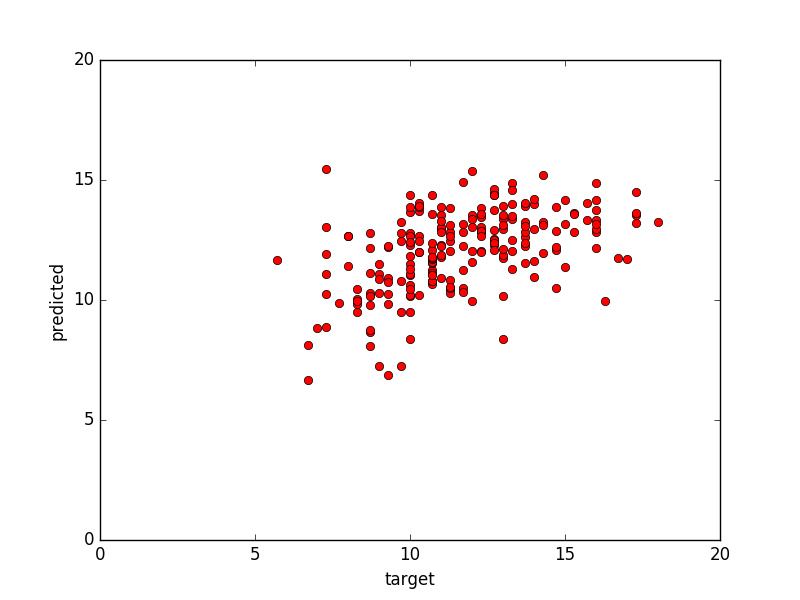
\includegraphics[width = 0.9\linewidth]{regression_test.png}
    \caption{Regression visualization showing predicted vs target values}
    \label{fig:fig1}
\end{figure}


\subsection{Artificial Neural Networks for Classification}
As previously mentioned, the classification part of the ANN implementation was done in Matlab, using its Pattern Recognition tool. Scaled conjugate gradient backpropagation was used as the learning algorithm, which tried to minimize the cross-entropy error. The multilayer perceptron neural network (MLP) had one hidden layer with 10 hidden neurons.

The following four tables show the results for the four tests. The first two tables include the confusion matrices from Matlab, while the second two tables contain the confusion matrices from Weka. 

\begin{table}[h!]
  \centering
  \begin{tabular}{l|cccccc}
     & \multicolumn{5}{c}{\textbf{Target Class}} \\ 
    \textbf{Output} & Fail & Sufficient & Satisfactory & Good & Very Good\\
    \hline
    Fail & 1 & 0 & 1 & 0 & 0\\ 
    Sufficient & 1 & 3 & 2 & 2 & 0\\ 
    Satisfactory & 22 & 34 & 73 & 47 & 24\\  
    Good & 20 & 49 & 82 & 98 & 49\\  
    Very Good & 3 & 4 & 10 & 40 & 69\\
  \end{tabular}
  \caption{Matlab implementation's confusion matrix for the 5-class problem.}
  \label{tab:table1}
\end{table}



\begin{table}[h!]
  \centering
  \begin{tabular}{c|cc}
    & \multicolumn{2}{c}{\textbf{Target Class}} \\ 
    \textbf{Output} & Below & Above \\ \hline 
     Below & 227 & 57\\ 
     Above & 102 & 248\\ 
  \end{tabular}
  \quad
  \begin{tabular}{c|cc}
    & \multicolumn{2}{c}{\textbf{Target Class}} \\
    \textbf{Output} & Below & Above\\ \hline
    Below & 244 & 95  \\
    Above & 85 & 210 \\
  \end{tabular}
  
  \caption{Left Table: Matlab implementation's confusion matrix for the binary problem. Right Table: Weka implementation's confusion matrix for the binary problem.}
  \label{tab:table1}
\end{table}

In Weka, the MLPClassify classifier function was used to perform the classifications. The following are the tables of classifications collected.

\begin{table}[h!]
  \centering
  \begin{tabular}{l|ccccc}
    & \multicolumn{5}{c}{\textbf{Target Class}} \\
    \textbf{Output} & Fail & Sufficient & Satisfactory & Good & Very Good\\ \hline
    Fail & 44 & 41 & 16 & 13 & 6\\
    Sufficient & 40 & 63 & 51 & 25 & 16\\
    Satisfactory & 18 & 50 & 58 & 38 & 25\\
    Good & 6 & 25 & 27 & 18 & 6\\
    Very Good & 8 & 11 & 17 & 6 & 6\\
  \end{tabular}
  \caption{Weka implementation's confusion matrix for the 5-class problem.}
  \label{tab:table1}
\end{table}

\begin{table}[h!]
  \centering
  \begin{tabular}{ccc}
  \hline
    \textbf{Implementation} & \textbf{5-class} & \textbf{Binary} \\
    \hline
    Matlab &  38.5 \%  & 74.8 \%  \\
    Weka  & 29.8 \% & 71.6 \%  \\
    \hline
  \end{tabular}
  \caption{Classification Accuracies for ANN Classification}
  \label{tab:table1}
\end{table}

\subsection{Decision Trees}

The decision trees were implemented both in Python using the sklearn library, and in Weka. The results and confusion matrices of these implementations are presented and compared in this section.

\subsubsection{Binary Classification}
For the binary classification, the Python sklearn classification was more accurate than the Weka implementation with 68.1 \% and 63.3 \% precision respectively. The confusion matrices are shown in table \ref{tab:DTbinary}.

\begin{table}[h]
\begin{center}
  \begin{tabular}{c|cc}
  & \multicolumn{2}{c}{\textbf{Target Class}} \\
 \textbf{Output} & Above & Below\\ \hline
  Above & 79 & 38 \\
  Below & 29 & 64
\end{tabular}
\quad
\begin{tabular}{c|cc}
  & \multicolumn{2}{c}{\textbf{Target Class}} \\
 \textbf{Output} & Above & Below\\ \hline
  Above & 64 & 53 \\
  Below & 24 & 69
\end{tabular}
\caption{Left table: Confusion matrix of sklearn implementation; Right table: Confusion matrix of Weka implementation }
\label{tab:DTbinary}
\end{center}
\end{table}

\subsubsection{Multilevel Classification}
For the 5-level classification, the sklearn implementation again achieved the best result with 33.8 \% accuracy, compared to the 31 \% accuracy of the Weka implementation. The confusion matrices of the sklean and Weka classifiers are shown in table \ref{tab:DT5level_sklearn} and \ref{tab:DT5level_weka} respectively.

\begin{table}[h]
  \begin{tabular}{l|ccccc}
     & \multicolumn{5}{c}{\textbf{Target Class}} \\ 
  \textbf{Output} & Very Good & Good & Satisfactory & Sufficient & Fail \\  \hline
  Very Good  & 5 & 3 & 4 & 3 & 1\\
     Good & 2 & 7 & 5 & 6 & 2\\
     Satisfactory & 8 & 16 & 15 & 12 & 4\\
     Sufficient & 5 & 9 & 18 & 25 & 14\\
     Fail & 2 & 7 & 8 & 10 & 19\\
  \end{tabular}
  \caption{Confusion matrix of sklearn implementation}
\label{tab:DT5level_sklearn}
\end{table}

\begin{table}[h]
  \begin{tabular}{l|ccccc}
     & \multicolumn{5}{c}{\textbf{Target Class}} \\ 
  \textbf{Output} & Very Good & Good & Satisfactory & Sufficient & Fail \\  \hline
  Very Good  & 1 & 4 & 8 & 2 & 1\\
     Good & 3 & 5 & 9 & 4 & 1\\
     Satisfactory & 7 & 19 & 16 & 7 & 6\\
     Sufficient & 5 & 13 & 16 & 20 & 17\\
     Fail & 1 & 3 & 7 & 12 & 23\\
  \end{tabular}
  \caption{Confusion matrix of Weka implementation}
\label{tab:DT5level_weka}
\end{table}

\subsection{Comparison of all algorithms and discussion of results}
Across the experiment, binary and five-class classifiers were successfully built for the dataset. However, classification accuracy of over 75\% on the binary classifier, and over 40\% on the five-class classifier was not achieved, as shown in table \ref{tab:ClassificationAccuracy}.\\

\begin {table}[h]
\begin{center}
  \begin{tabular}{lllll}  
    \hline
   \textbf{Classification} & \textbf{ANN} & \textbf{kNN} & \textbf{DT} \\ \hline
    5-class & 38.5 \% & 33 \% & 34 \% \\
    binary & 74.8 \% & 61 \% & 68 \% \\
    \hline
  \end{tabular}
  \caption{Classification Accuracy}
 \label{tab:ClassificationAccuracy}
\end{center}
\end{table}

As can be expected from these results, none of these algorithms can make perfect (or probably even reliable) classifications or regressions from the data set. Among the three algorithms, the artificial neural network proved to be the most accurate, with a five-class of 38.5\% and a binary reaching almost 75\%. Referring back to the inividual discussion of each algorithm, with all of the from-scratch implementations of the algorithms explored, it can be found that each one reaches conclusions relatively close to that found by the Weka implementations. This closeness in results reveals that the algorithms implemented may be sufficient and reliable under normal circumstances, and show that the lack of accuracy in classification can be found in other areas.

This aforementioned lack of accuracy can most likely be found in the sourced data set itself. This may be due to:
    \begin{itemize}
        \item The data set not being big enough (649 records). Simply put, more students need to be gathered for this set.
        \item The data set features not having a large enough influence on the classes, more specifically an attribute cannot reliably contribute towards the classification of a student.
        \item The attributes used in this data set may not have been the best in terms of accurately relating to student performance.
        \item The timespan of data collected may not be broad enough: only one school year was covered in two public schools. This may be rectified by sourcing data across multiple school years or gathering data from across the region.
    \end{itemize}  

%\input{discussion}
% We don't need a seperate discussions section. Everything can be explained in the results and conclusion chapters
\section{Conclusion}
This experiment attempted to use academic and demographic records from students taking two subjects in two schools in Portugal to classify and extrapolate the average grade of a student. This data set was first preprocessed based on sound principles reducing the number of outliers in the set, then subsequently mined using custom and provided implementations of the linear regression, naïve Bayes classification, k-Nearest Neighbor, artificial neural networks, and decision trees algorithms. However, due to the quality of the data set itself, accurate classifiers were not able to be constructed, only at most giving an accuracy of 75\% in the best case. As a result of the inability to generate relatively accurate classifiers, it is not yet possible to begin to envision effective manners of improving student education based on their demographic information.

\bibliographystyle{abbrv}
\bibliography{bibliography}

%data set:
%insufficient information
%other factors more influence
%further:
%development of grades over lifetime
%impact of social influences over the time
%

\end{document}
